\documentclass[aspectratio=169]{beamer}


\usepackage[utf8]{inputenc}
\usepackage{amsmath}
\usepackage{amsfonts}
\usepackage{amssymb}
\usepackage{graphicx}
\usepackage{ragged2e}  % `\justifying` text
\usepackage{booktabs}  % Tables
\usepackage{tabularx}
\usepackage{tikz}      % Diagrams
\usetikzlibrary{calc, shapes, backgrounds}
\usepackage{amsmath}
\usepackage{amssymb}
\usepackage{dsfont}
\usepackage{url}       % `\url
\usepackage{listings}  % Code listings
\usepackage[T1]{fontenc}
\usepackage{hyperref}
\usepackage{theme/beamerthemehbrs}

\author[Dashboard for ROS-based System]{}
\title{Software Development Project}
\subtitle{Dashboard for ROS-based System}
\institute[HBRS]{Hochschule Bonn-Rhein-Sieg}
\date{\today}
\subject{Test beamer}

% \thirdpartylogo{path/to/your/image}


\begin{document}
{
\begin{frame}
\titlepage
\end{frame}
}

\begin{frame}{Team Members}
\linespread{2}
\vspace*{-20mm}
	\begin{enumerate}
	\item \bf{Lokesh Veeramacheneni}
	\item \bf{Zuha Karim}
	\item \bf{Anargh Viswanath}
	\end{enumerate}
	\vspace*{5mm}
	%In the current stage of the project, the team members are yet to assume separate roles.\\ 
%\vspace*{2.5mm}	
	Currently all members are working as developers.\\
	
\end{frame}

\begin{frame}{Project Objective}
\vspace*{-15mm}
\justify \bf{Developing a Dashboard UI for monitoring the ROS system running on a robot remotely through a computer system via web services.}
\end{frame}

\begin{frame}{Client and  Dashboard Features}
\vspace*{-15mm}
\linespread{1.5}
\bf Client: \textnormal{Deebul Nair}\\
\textnormal{It is intended to be used by \bf{Robocup @work lab}.}

	\textnormal{Features offered by the Dashboard:}
	\begin{enumerate}
	\item \textnormal{Effortless visualization of ROS Nodes.}
	\item \textnormal{Smooth monitoring of ROS and Robot's system metrics.}
	\item \textnormal{Start and kill the ROS nodes.(if possible)}
	\end{enumerate}
	
\end{frame}

\begin{frame}{Main Components}
\vspace*{-10mm}
\linespread{1.5}
\begin{enumerate}
	\item \textbf{Cockpit} - Integrated open web-based interface for GNU/Linux server.\\ \textbf{Features of Cockpit:}
	\begin{itemize}
	\item Monitor and administer several servers at the same time.
	\item Uses the system’s normal user logins and privileges by default. 
	\item Network login supported.
	\item When inactive, no extra load on the server.
	\item Inbuilt packages show the status of the system.
	\item Embedded terminal present within interface.
	\end{itemize}
	\item \justify \textbf{ROS Kinetic} - Installed on the robot which has to be monitored.
\end{enumerate}
	
\end{frame}

\begin{frame}{Coding standards}
\vspace*{-25mm}
\linespread{2}
\begin{enumerate}
	\item \textbf{Python}
	\begin{itemize}
	\item PEP8
	\end{itemize}
	\item \textbf{Javascript}
		\begin{itemize}
	\item Google JavaScript Style Guide
	\end{itemize}
\end{enumerate}
	
\end{frame}

\begin{frame}{Organization of Work}
\vspace*{-15mm}
\linespread{2}
	\begin{itemize}
	\item Currently the project management is being carried ouut through Github.
	\item Each member has a separate branch for development.
	\item Master branch is having the reviewed components merged from branches.
	\item Issues, Sprints and progress also being placed.
	\item  \href{https://github.com/lokeshveeramacheneni/Software-Development-Project/tree/master}{\underline{Link to Github Repository.}} 
	\item Alternatives to Github such as Jira being considered.
	\end{itemize}
	
\end{frame}
\begin{frame}{Proposed Pipeline of Project}
\begin{figure}
  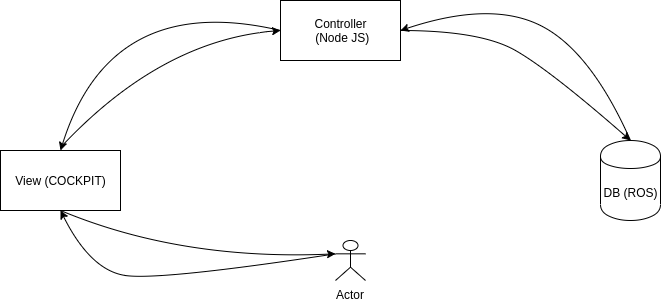
\includegraphics[width=0.8\linewidth]{pipeline.png}
  \caption{MVC Pattern}
  \label{fig: MVC Pattern}
\end{figure}
\end{frame}
\begin{frame}{Current stage of work}
\vspace*{-15mm}
\linespread{1.5}
	\textbf{Description of terms}
	\begin{itemize}
\item rosbridge - package providing JSON API to ROS functionality for non-ROS programs.
\item websocket - protocol to establish stable connection between Client and Server.
\item roslib - base dependencies and support libraries for ROS.
	\end{itemize}
\end{frame}

\begin{frame}{Current stage of work}
\vspace*{-10mm}
\linespread{1.5}
	\textbf{Connecting Html to ROS}
	\begin{enumerate}
\item Json files are used to establish a connection with ROS through web browser via websockets.
\item Created a ROS node and connected it to local host port 9091.
\item Added a listner, publisher and displayed the result on html page.
\item Used roslib objects  and functions for subscribing and listening to a topic.
\item Successful in connecting html with ros using rosbrige and roscore.
\item \textit{ More detailed work has to be carried out.}
	\end{enumerate}
\end{frame}

\begin{frame}{Current stage of work}
\begin{figure}
  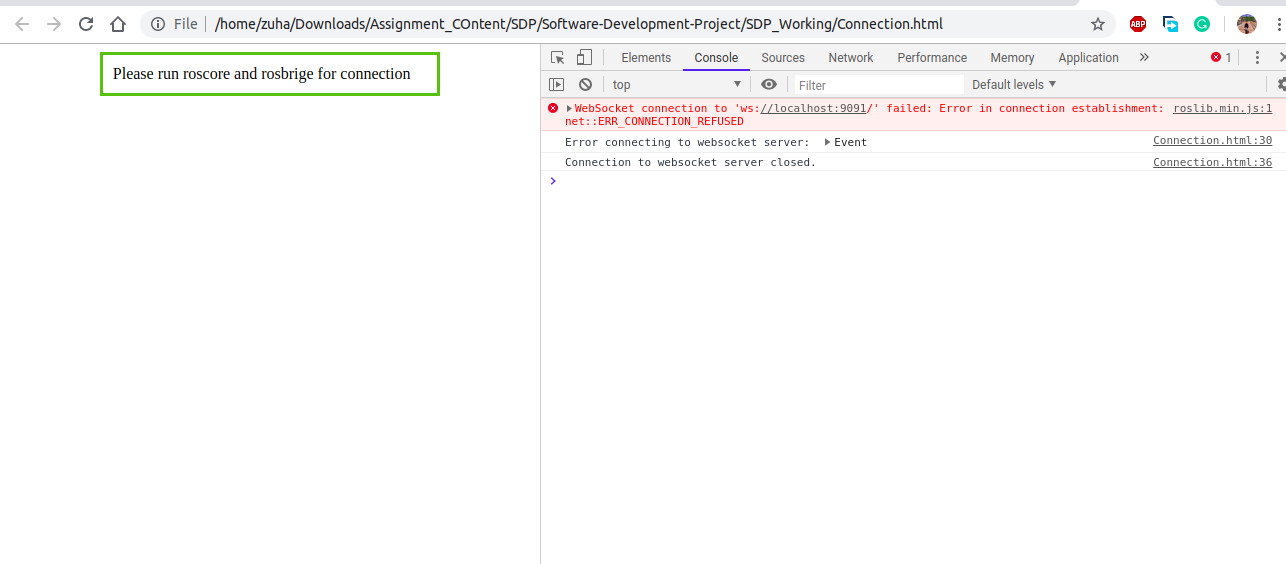
\includegraphics[width=0.8\linewidth]{notConnected.png}
  \caption{Not connected}
  \label{fig:Not Connected}
\end{figure}
\end{frame}

\begin{frame}{Current stage of work}
\begin{figure}
  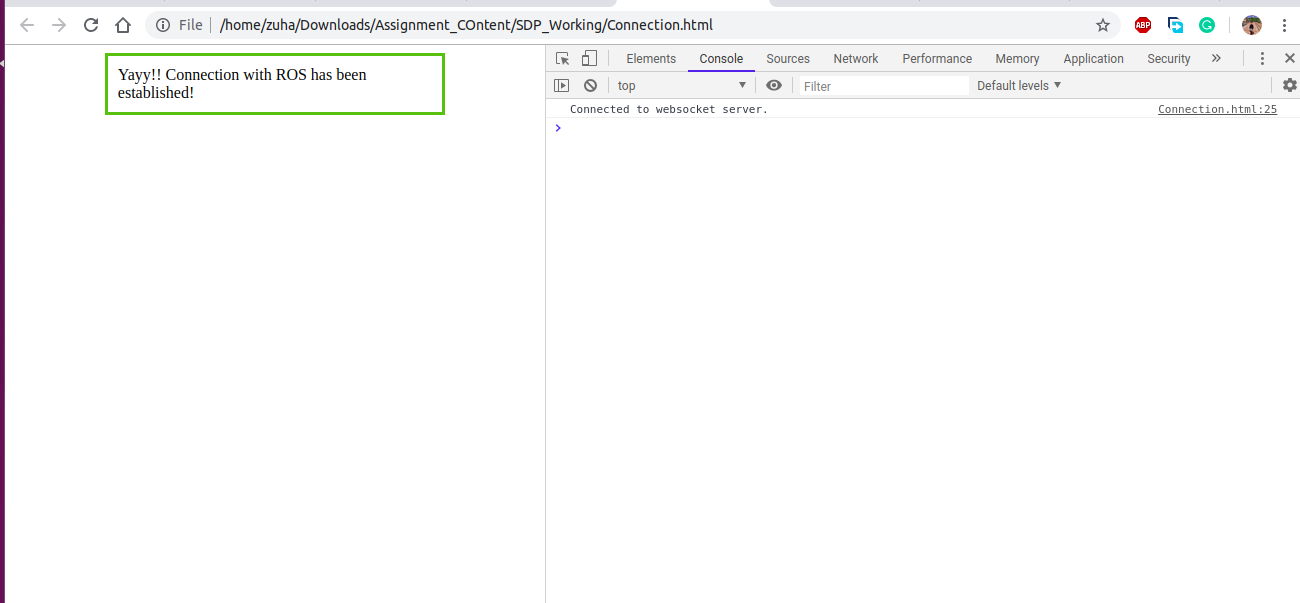
\includegraphics[width=0.8\linewidth]{Connection.png}
  \caption{Successful connection}
  \label{fig:Connected}
\end{figure}
\end{frame}

\begin{frame}{Course of action for upcoming week}
\vspace*{-15mm}
\linespread{2}
	\begin{itemize}
	\item Start Sprint 1 (2-3 weeks)
	\item Assign Userstories and work on them
	\end{itemize}
\end{frame}

\end{document}
